\documentclass[12pt, a4paper, oneside]{ctexbook}
\usepackage{amsmath, amsthm, amssymb, bm, graphicx, mathrsfs}
\usepackage{geometry}
\usepackage{listings,xcolor}
\usepackage{pdfpages}
\usepackage{hyperref}

%设置引用格式
\hypersetup{
	colorlinks=true,linkcolor=black,colorlinks=true,linkcolor=black,citecolor=blue,urlcolor=blue
}

%代码配置
\lstset{
	breaklines,%自动换行
	columns=fixed,       
	numbers=left,                                        % 在左侧显示行号
	frame=none,		                                     % 不显示背景边框
	backgroundcolor=\color[RGB]{245,245,244},            % 设定背景颜色
	keywordstyle=\color[RGB]{40,40,255},                 % 设定关键字颜色
	numberstyle=\footnotesize\color{darkgray},           % 设定行号格式
	commentstyle=\it\color[RGB]{0,96,96},                % 设置代码注释的格式
	stringstyle=\rmfamily\slshape\color[RGB]{128,0,0},   % 设置字符串格式
	showstringspaces=false,                              % 不显示字符串中的空格
	language=C,                                          % 设置语言
	tabsize=2,
}

\CTEXsetup[format={\Large\bfseries}]{section}	%section 居左(默认居中)

%配置纸张边缘
\geometry{left=2.54cm,right=2.54cm,top=3.18cm,bottom=3.18cm}

\title{{\Huge{\textbf{实现函数说明文档}}}\normalsize{\\——第六届全国大学生集成电路创新创业大赛景嘉微杯初赛提交文档}}
\author{队名:虹ヶ咲学园芯片设计同好会\\ 成员:黄金源\space邓立唯\space林明锋}
\date{\today}
\linespread{1.5}


\begin{document}
%-----------------------封面------------------
	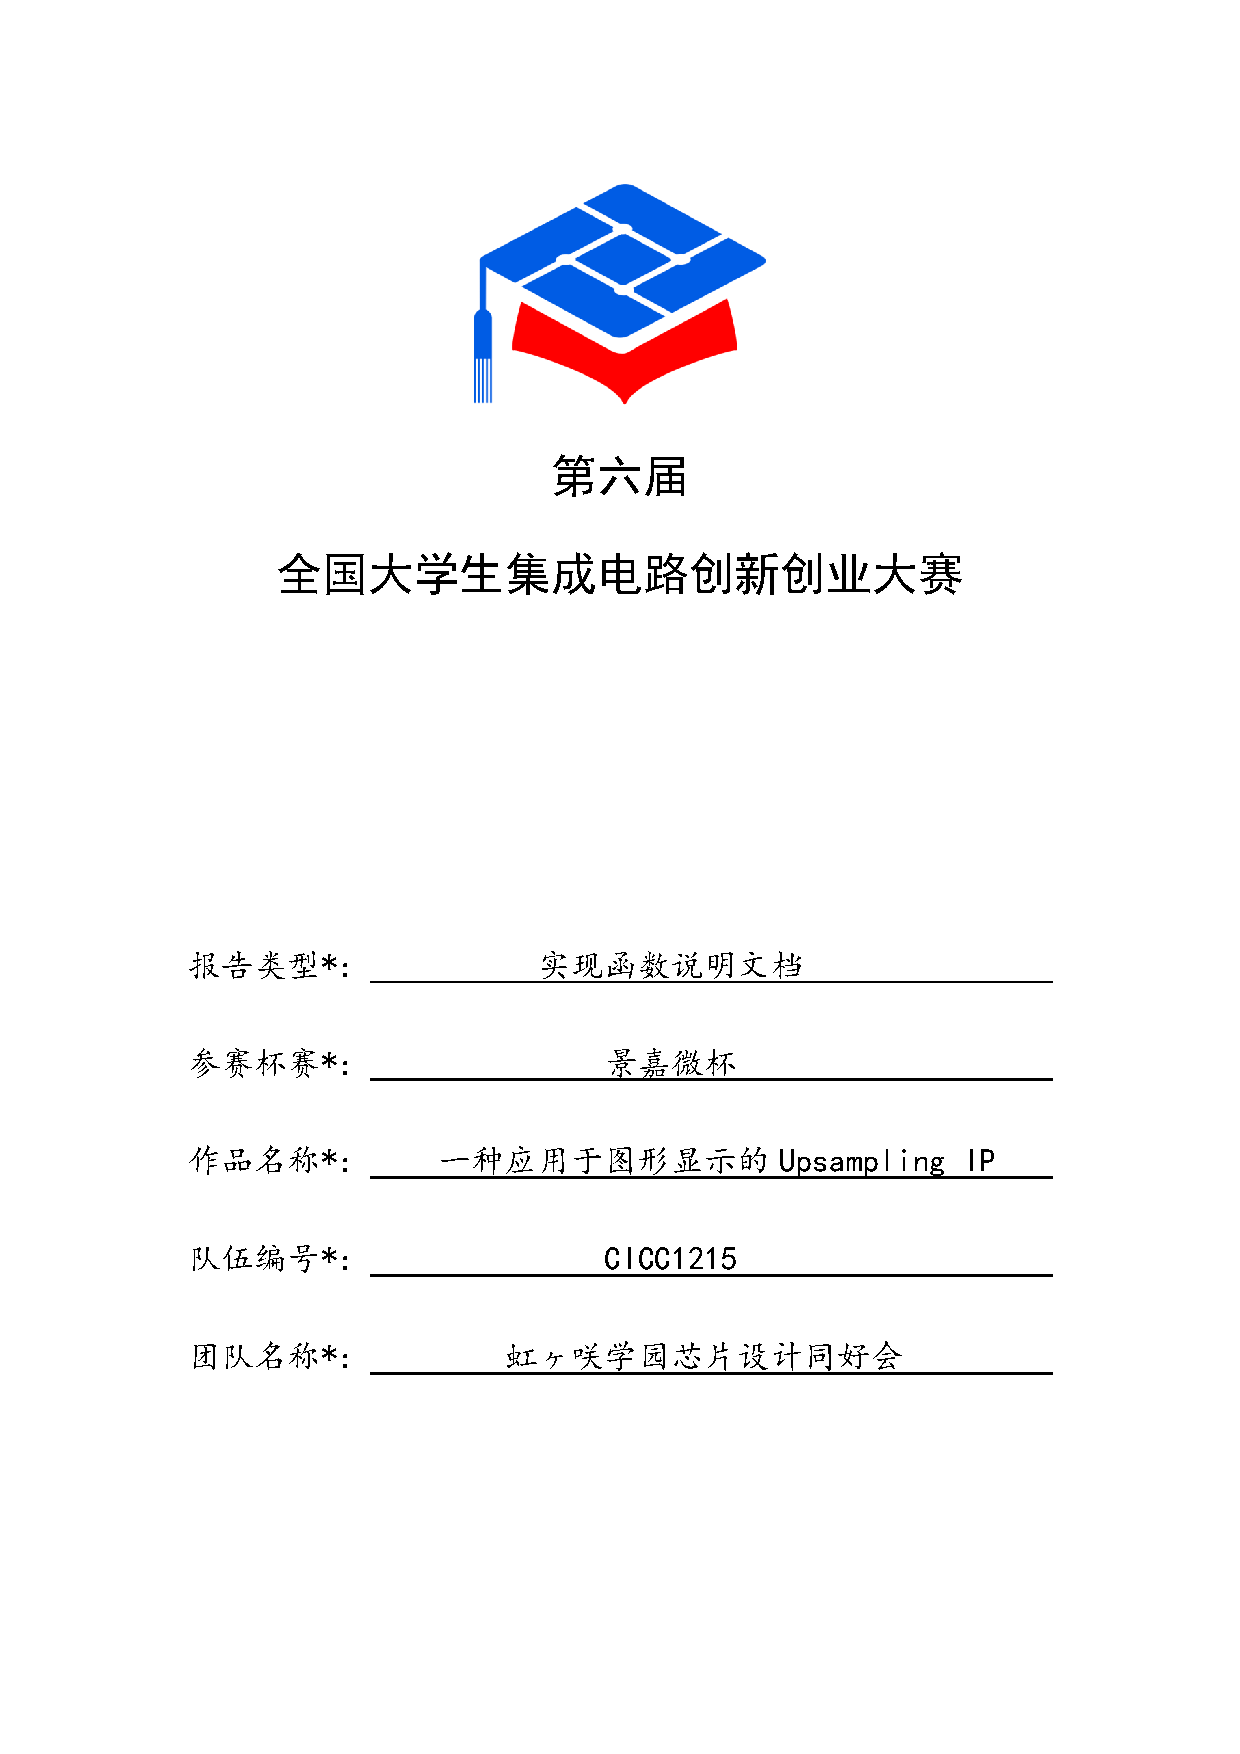
\includepdf{./pic/cover.pdf}
	\maketitle	
	\pagenumbering{Roman}
	\setcounter{page}{1}
%-----------------------前言------------------
	\begin{center}
		\Huge\textbf{前言}
	\end{center}~\

本文档( 函数现函数说明文档)仅作为虹ヶ咲学园芯片设计同好会(成员:黄金源、邓立唯、林明锋)参加第六届全国大学生集成电路创新创业大赛景嘉微杯赛初赛提交文档供评委评分使用。
	~\\
	\begin{flushright}
		\begin{tabular}{c}
			虹ヶ咲学园芯片设计同好会\\
			\today
		\end{tabular}
	\end{flushright}
%-----------------------目录------------------
	\newpage
	\pagenumbering{Roman}	%Roman or arabic
	\setcounter{page}{1}
	\tableofcontents
	\newpage
	\setcounter{page}{1}
	\pagenumbering{arabic}
	
%-----------------------正文----------------	
	\chapter{基本介绍}
	\section{整体流程}
		\begin{figure}[h]
			\centering
			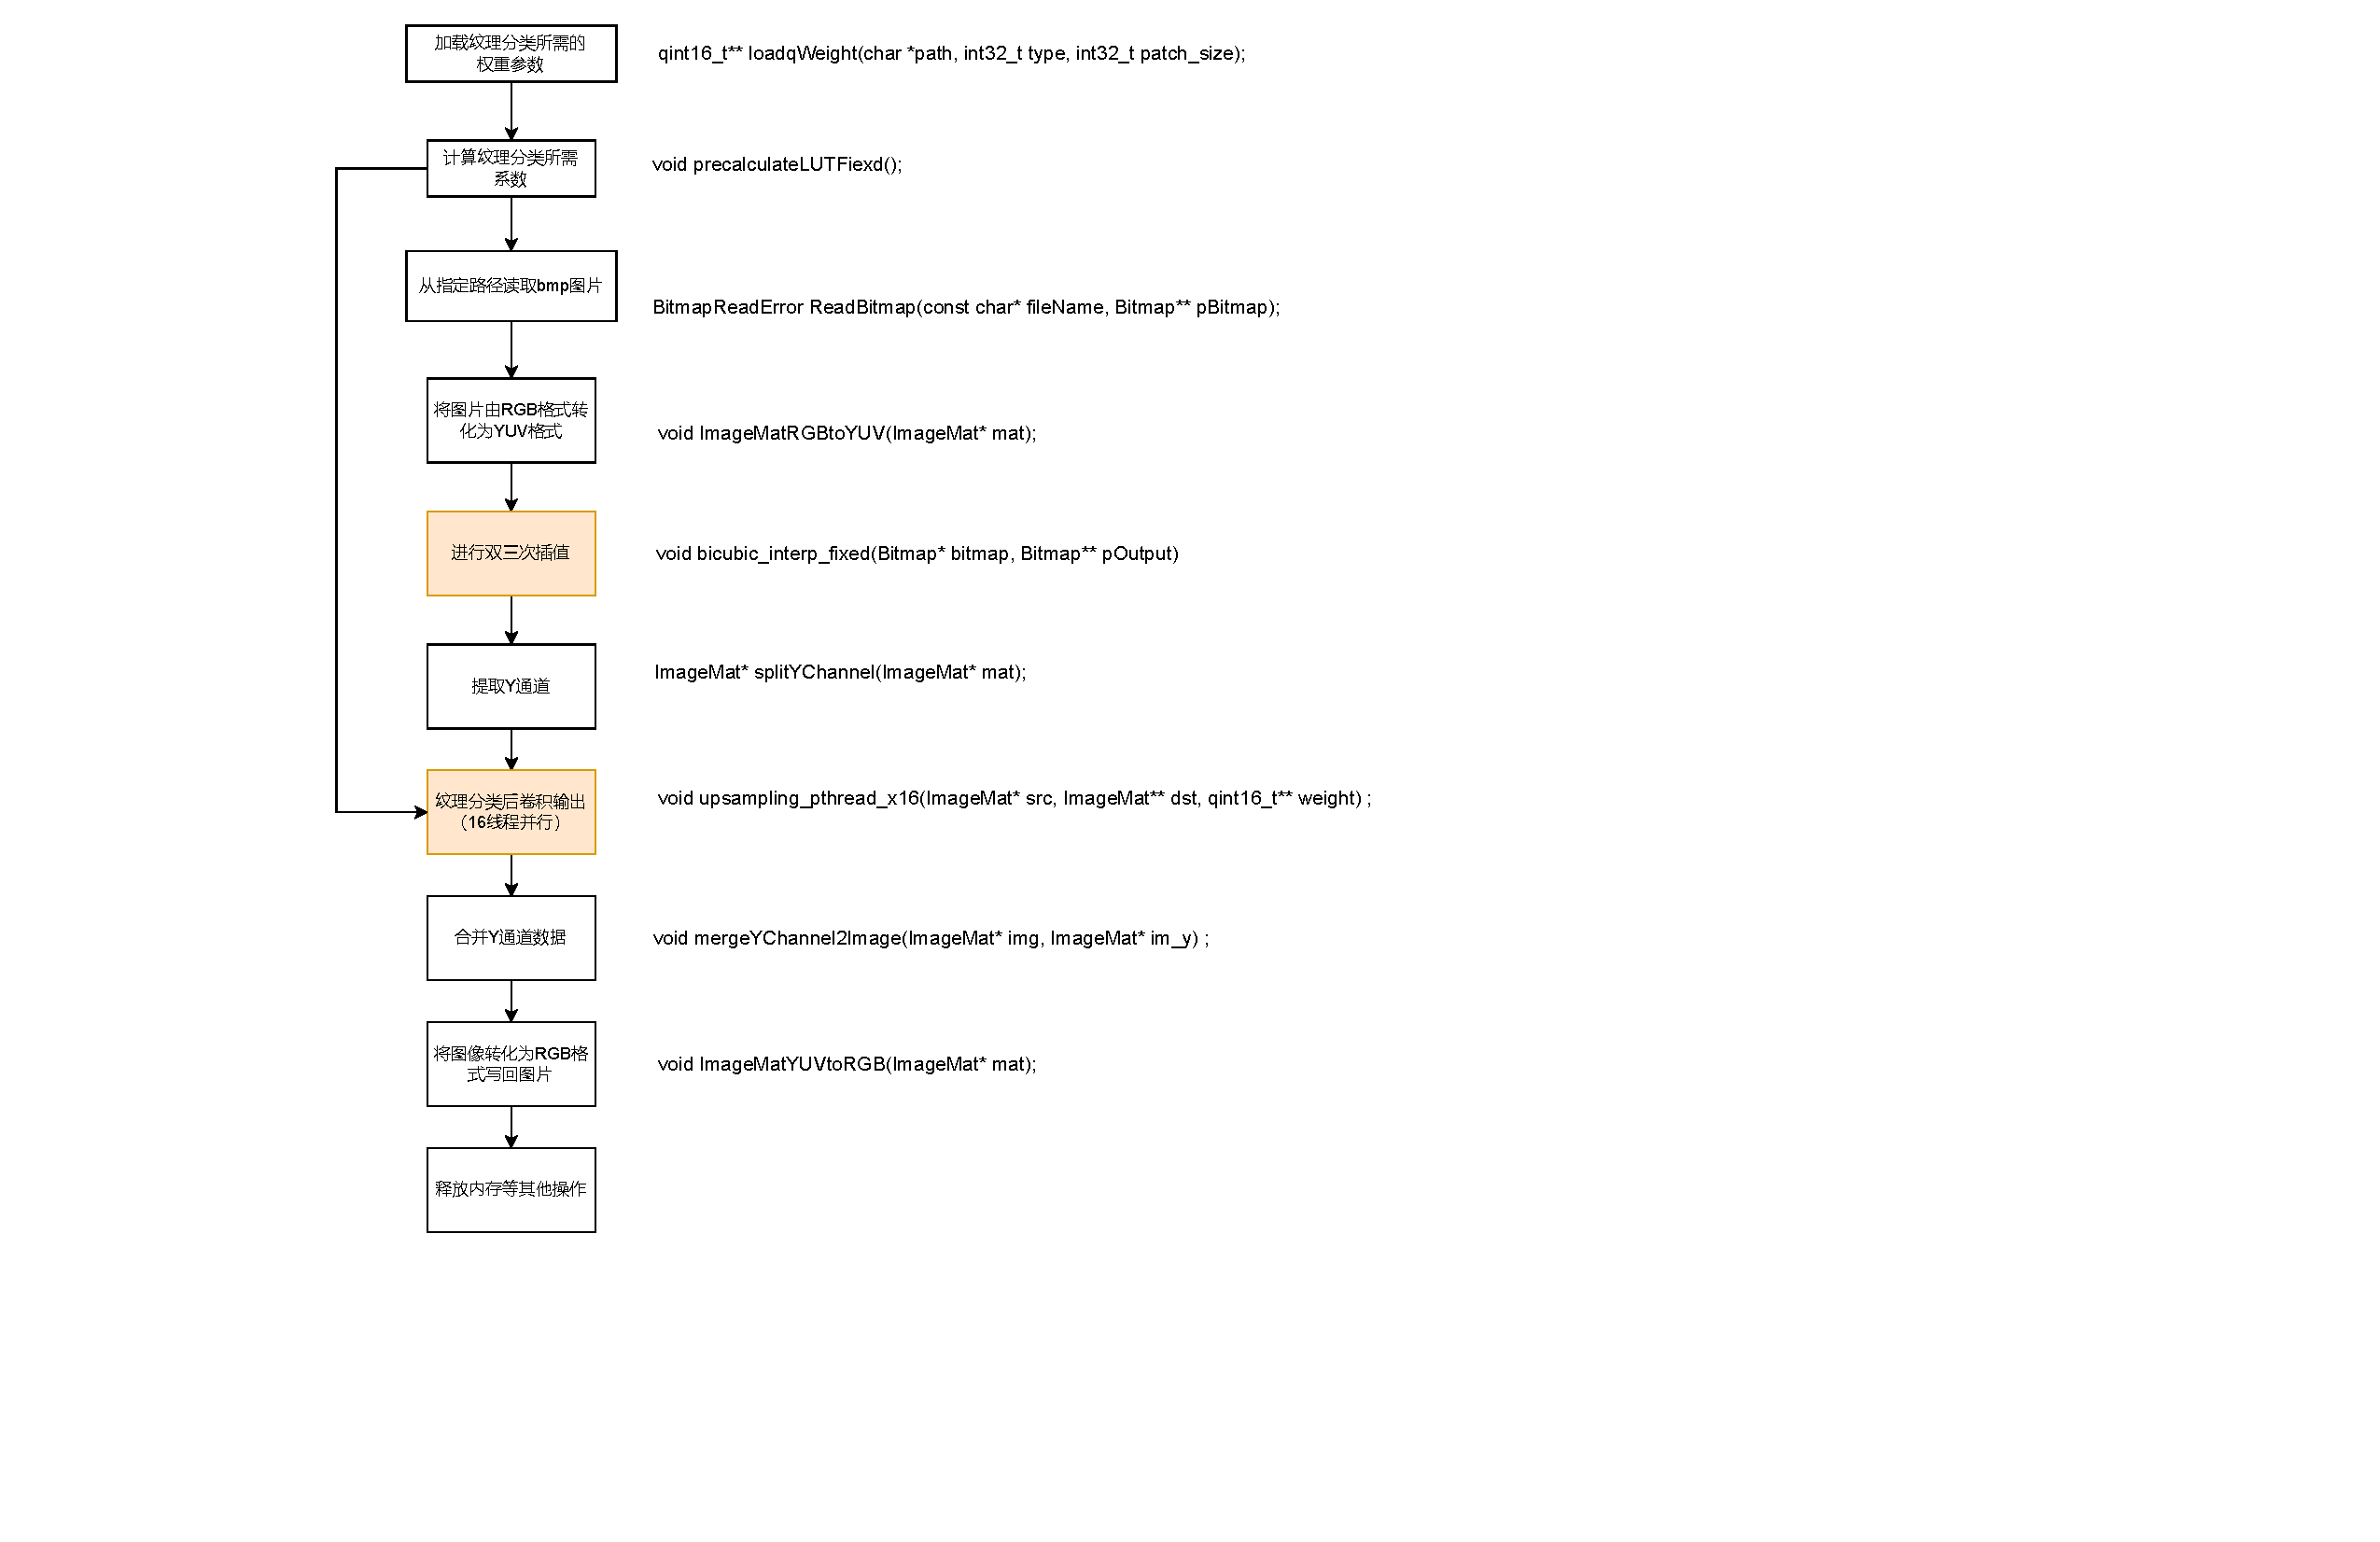
\includegraphics[scale=0.65]{pic/overview}
			\caption{程序整体流程}
			\label{fig:overview}
		\end{figure}
	\section{数据结构}
		\subsection{图片格式}
		\begin{enumerate}
			\item \textbf{BitmapHead:}包含bmp文件信息头各个信息相对于文件头的偏移量
			\begin{lstlisting}
typedef struct {
	uint32_t biSize;
	uint32_t biWidth;
	uint32_t biHeight;
	uint16_t biPlanes;
	uint16_t biBitCount;
	uint32_t biCompression;
	uint32_t biSizeImage;
	uint32_t biXPelsPerMeter;
	uint32_t biYPelsPerMeter;
	uint32_t biClrUsed;
	uint32_t biClrImportant;
}BitmapHead;
			\end{lstlisting}
			
			
			\item \textbf{Bitmap:}包含bmp图像的文件信息:文件名、文件信息头结构体指针和图像数据指针
			\begin{lstlisting}
typedef struct {
	char* fileName;
	BitmapHead *head;
	ImageMat *image;
}Bitmap;
			\end{lstlisting}
			
			
			\item \textbf{ImageMat:} 包含图像的宽度、高度和数据所在的内存首地址
			\begin{lstlisting}[numbers=none]
typedef struct {
	int width;
	int height;
	uint8_t *pData;
}ImageMat;		
			\end{lstlisting}			
		\end{enumerate}
		
		\subsection{量化}
		\begin{enumerate}
			\item \textbf{qint16\_t:}带量化位数的16位变量类型,real表示变量真实值,Qn表示该变量需要量化的位数
				\begin{lstlisting}
typedef struct {
	int16_t real;		
	uint8_t Qn;			
}qint16_t;					
				\end{lstlisting}
			\item \textbf{qint32\_t:}带量化位数的32位变量类型,real表示变量真实值,Qn表示该变量需要量化的位数
				\begin{lstlisting}
typedef struct {
	int32_t real;	
	uint8_t Qn;		
}qint32_t;				
			\end{lstlisting}
			\item \textbf{qImageMat:}带量化位数的图像数据存储格式
				\begin{lstlisting}
typedef struct {
	int width;
	int height;
	qint16_t* pData;
}qImageMat;			
			\end{lstlisting}
			\item \textbf{QuantizeError:}量化运算成功或失败标志
				\begin{lstlisting}
typedef enum {
	OK = 0,
	QN_ALARGE,
	QN_BLARGE
}QuantizeError;		
			\end{lstlisting}
			\item \textbf{qCompareRes:}量化比较结果
				\begin{lstlisting}
typedef enum {
	Q_EQ = 0,	
	Q_GR,     // >
	Q_LT      // <
}qCompareRes;		
				\end{lstlisting}
			
		\end{enumerate}

	
	
	
	
	
	\chapter{实现函数细节}	
%%--------------------双三----------------	
	\section{超分辨率实现}
	\begin{enumerate}
		\item \textbf{双三次插值}
		\begin{lstlisting}[numbers=none]
void bicubic_interp_fixed(Bitmap* bitmap, Bitmap** pOutput);
		\end{lstlisting}
		\textbf{参数:} \par bitmap: 要进行双三次插值的图像 \par pBitmap: Bitmap类型的指针变量,用于存储fileName的文件信息 \\
		\textbf{返回值:}\par 无返回值\\
		\textbf{作用:}\par 对输入图像进行双三次插值,提高图像分辨率\\
	
	\item \textbf{上采样——多线程实现}
		\begin{lstlisting}[numbers=none]
void upsampling_pthread_x16(ImageMat* src, ImageMat** dst, qint16_t** weight);			
		\end{lstlisting}
		\textbf{参数:} \par src: 要进行采样的图像 \par dst: 上采样后得到的图像\par weight: 带有量化位数的权重\par
		\textbf{返回值:}\par 无返回值\\
		\textbf{作用:}\par 对输入图像进行双三次插值,提高图像分辨率\\
		\textbf{说明:}\par 在本次设计中,需要先根据patch\_edge进行图像分类,再将图像的patch 和 patch\_edge 一一对应,执行相应计算。本次设计中,需要处理4k分辨率图像,采用顺序执行的方式非常耗费时间,因此该函数采用了并行计算的方式,先将待处理图像分为4×4共计16个部分,创建16个线程并行计算,等待16个线程返回后再执行下一步计算,大大提高了运行速率。

		
	\end{enumerate}
	

		
%%--------------------锐化----------------	
	\section{锐化}
%%--------------------其余组件----------------	
	\section{其余组件}
		\subsection{内存管理}
		\begin{lstlisting}[numbers=none]
void freeqWeightSpace(qint16_t ** weight, int32_t type);
		\end{lstlisting}
	\textbf{参数:} \par weight : qint\_16 类型的指针 \par type: int32\_t 类型的变量 \\
	\textbf{返回值:}\par 无返回值 \\
	\textbf{作用:}\par 用于释放申请的内容空间\\
	
	
		\subsection{图片读取与格式转换}
		\begin{enumerate}
			\item \textbf{ReadBitmap}——读取bmp格式图片
				\begin{lstlisting}[numbers=none]
BitmapReadError ReadBitmap(const char* fileName, Bitmap** pBitmap);
				\end{lstlisting}
				\textbf{参数:} \par fileName: 要读取的bmp格式图片路径 \par pBitmap: Bitmap类型的指针变量,用于存储fileName的文件信息 \\
				\textbf{返回值:}\par BitmapReadError 类型的枚举变量,用于表示读取文件是否成功\\
				\textbf{作用:}\par 用于读取bmp格式图片\\
			
			\item \textbf{WriteBitmap}——写bmp格式图片
				\begin{lstlisting}[numbers=none]
BitmapWriteError WriteBitmap(Bitmap* bitmap, const char* fileName);
				\end{lstlisting}
				\textbf{参数:} \par fileName: 要写入的bmp格式图像路径 \par bitmap: Bitmap类型的指针变量,用于存储fileName的文件信息 \\
				\textbf{返回值:}\par BitmapWriteError 类型的枚举变量,用于表示写入文件是否成功\\
				\textbf{作用:}\par 用于写bmp格式图像\\
			
			\item \textbf{ImageMatRGBtoYUV}——将RGB编码图片转换为YUV编码图片
				\begin{lstlisting}[numbers=none]
void ImageMatRGBtoYUV(ImageMat* mat);
				\end{lstlisting}
				\textbf{参数:} \par mat: ImageMat类型的结构体指针,用于存储图像的长度、宽度和数据信息\par 
				\textbf{返回值:}\par 无返回值 \\
				\textbf{作用:}\par  将RGB编码图片转换为YUV编码图像\\

			\item \textbf{ImageMatYUVtoRGB}——将YUV编码图片转换为RGB编码图片
				\begin{lstlisting}[numbers=none]
void ImageMatYUVtoRGB(ImageMat* mat);
				\end{lstlisting}
				\textbf{参数:} \par mat: ImageMat类型的结构体指针,用于存储图像的长度、宽度和数据信息\par 
				\textbf{返回值:}\par 无返回值 \\
				\textbf{作用:}\par  将YUV编码图像转换为RGB编码图像\\
			
			
			\item \textbf{ImageMatRGBtoYUV}——提取YUV编码格式中Y通道数据
				\begin{lstlisting}[numbers=none]
ImageMat* splitYChannel(ImageMat* mat);
				\end{lstlisting}
				\textbf{参数:} \par mat: ImageMat类型的结构体指针,用于存储图像的长度、宽度和数据信息\par 
				\textbf{返回值:}\par ImageMat 类型指针,存储图片的长度、宽度和YUV编码格式中Y通道数据 \\
				\textbf{作用:}\par 提取YUV编码格式中Y通道数据 \\

			\item \textbf{mergeYChannel2Image}——将YUV编码格式中Y通道数据合并到图像中
				\begin{lstlisting}[numbers=none]
void mergeYChannel2Image(ImageMat* img, ImageMat* im_y);
				\end{lstlisting}
				\textbf{参数:} \par mat: 要合并的目标图像,ImageMat类型的结构体指针,用于存储图像的长度、宽度和数据信息\par im\_y:ImageMat 类型指针,存储要合并图像的长度、宽度和Y通道数据信息 \\
				\textbf{返回值:}\par 无返回值 \\
				\textbf{作用:}\par 将YUV编码格式中Y通道数据合并到图像中 \\			

			\item \textbf{DestoryImageMat}——释放图像内存空间
				\begin{lstlisting}[numbers=none]
void DestoryImageMat(ImageMat* mat);
				\end{lstlisting}
				\textbf{参数:} \par mat: ImageMat 类型的结构体指针,用于存储图像的长度、宽度和数据信息\par 
				\textbf{返回值:}\par 无返回值 \\
				\textbf{作用:}\par 内部调用 free 释放申请的图像内存 \\					
		\end{enumerate}
		
		\chapter{最终效果}
		
		\begin{figure}[h]
			\centering
			
\includegraphics[width=0.7\linewidth]{pic/test}
			\caption{}
			\label{fig:test}
		\end{figure}


	
	
\end{document}